\chapter{Medžiagų elektrinis laidumas.}

\section{Elektros srovės nešėjų metaluose prigimtis}

Pirmasis jau 1901 metais elektros srovės nešėjų metaluose prigimtį
bandė eksperimentiškai nustatyti Rikke. Jis dirbo jau žinodamas
Faradėjaus dėsningumus. (Faradėjus parodė, kad elektrolituose
krūvį perneša jonai.) Rikke hipotezė buvo, kad krūvį metaluose
irgi perneša jonai.  Jis sujungė strypus, taip kaip parodyta TODO:
Paveikslėlis iš 46 skaidrės ir leido jais tekėti visus metus
nuolatinę srovę. Per šį laiką pratekėjo $3,5\cdot 10^{6}C$
krūvis, tačiau nei strypų svoris, nei sąlyčio taškai nepakito.
Rikke padarė išvadą, kad medžiagos atomai metaluose srovės
pernešimo procesuose nedalyvauja ir iškėlė hipotezę, jog
tai gali būti elektronai, kuriuos 1897 metais atrado Tomsonas.

Norint tuo įsitikinti, reikėjo išmatuoti elektronų ženklą bei
savitąjį krūvį. Buvo sumanytas eksperimentas, kurio idėja rėmėsi
tuo, kad jeigu krūvio nešėjai metaluose yra elektronai,
tai privertus judėti strypą tam tikru greičiu (pažymėkime jį
$v_{0}$) ir tada jį staigiai stabdant jame turi atsirasti srovės
impulsas. (Nes elektronai iš inercijos juda toliau.) Beje, tokį
elektros krūvių pagreitį nejudančiame metalo cilindre galime
sudaryti patalpinę laidininką į elektrinį lauką:
\begin{equation*}
  E = -\frac{ma}{q},
\end{equation*}
tai yra prie jo galų prijungti įtampą:
\begin{align*}
  U &= lE \\
  I &= \frac{U}{R} \\
  dq
  &= Idt \\
  &= -\frac{lma}{eR}dt \\
  &= -\frac{m}{e}\frac{l}{R}dv, \\
\end{align*}
čia:
\begin{description}
  \item[$E$] – elektrinio lauko stipris;
  \item[$m$] – elektrono masė;
  \item[$a$] – strypo stabdymo pagreitis;
  \item[$q$] – strypu pratekėjęs elektros krūvis;
  \item[$e$] – elektrono krūvis;
  \item[$U$] – įtampa tarp strypo galų;
  \item[$l$] – strypo ilgis;
  \item[$I$] – srovės stipris;
  \item[$R$] – strypo varža;
  \item[$q$] – pratekėjęs krūvis;
  \item[$v$] – greitis FIXME: Kieno?
\end{description}

Stabdant strypu pratekės krūvis:
\begin{align*}
  q
  &= \int _{0} ^{t} dq \\
  &= -\int ^{0} _{v_{0}} \frac{ml}{eR}d\vec{v} \\
  &= \frac{m}{e} \frac{l\vec{v}}{R} \\
\end{align*}

Pirmieji tokį bandymą 1913 metais atliko Mandelštanas ir Papaleksi.
Dėl per didelių paklaidų, jų atsakymas buvo „gal“.

1916 metais Tomsonas ir Stiurtas ritę, su užvyniotu 500 metrų ilgio
laidininku, įsukę $300\frac{m}{s}$ linijiniu greičiu stabdė ir
paskaičiavo savitąjį krūvį $\left( \frac{q}{m} \right)$. Jie
gavo šį santykį, eksperimento paklaidų leistinuose rėmuose,
artimą elektrono savitajam krūviui:
\begin{equation*}
  \frac{\t{elektrono krūvis}}{\t{elektrono masė}}
  = \frac{1,6 \cdot 10^{-19}C}{9,109\cdot10^{-31}kg}
  = 1,756\cdot10^{11}\frac{C}{kg}.
\end{equation*}

Elektronų skaičių tūrio vienete galime apskaičiuoti pagal formulę:
\begin{equation*}
  n = \frac{\rho}{\mu}N_{A},
\end{equation*}
čia:
\begin{description}
  \item[$\rho$] – medžiagos tankis;
  \item[$\mu$] – kilomolio masė;
  \item[$N_{A}$] – Avogadro skaičius.
\end{description}

Klasikinė metalų laidumo teorija buvo pateikta Drudės, o vėliau
tikslinta Lorenco. Drudės modelis paaiškina, kodėl metalai nėra
neigiamai įelektrinti. Pagal jį, metalai yra kristalai, jų
elementariąją kristalinę gardelę sudaro katijonai, taigi teigiamai
įelektrinti jonai. Tačiau, tai yra tik indas į kurį talpinami
elektronai. Kiekvieną katijoną atitinka elektronas. Tokiu būdu
kadangi katijonas turi teigiamą krūvį, o elektronas – neigiamą,
šis krūvių konglomeratas yra subalansuotas ir medžiaga yra neutrali
elektriškai.

Pagal Drudę, vidutinis elektronų greitis metaluose gali būti išreikštas
lygtimi:
\begin{equation*}
  \bar{v} = \sqrt{\frac{8kT}{\pi m}},
\end{equation*}
taigi $T = 300 K$ temperatūroje
$\bar{v} \approx \sqrt{\frac{8\cdot1,38\cdot10^{-23}\cdot300}%
{3,14\cdot9,1\cdot10^{-31}}} \approx 10^{5} \frac{m}{s}$. Jeigu
talpiname metalą į elektrinį lauką, tai be chaotinio judėjimo greičio
$\bar{v}$ dar atsiranda ir tvarkingas greitis $v_{t}$.

Tarkime, jog elektronas iki susidūrimo vidutiniškai nuskrieja atstumą
$l$ (dydis $l$ vadinamas elektrono laisvuoju lėkiu). Jis tą
atstumą įveikia per savo laisvojo lėkio laiką:
\begin{equation*}
  \tau = \frac{l}{\vec{v}}.
\end{equation*}
Elektrinis laukas, į kurį yra patalpintas metalas, elektroną veikia
jėga:
\begin{equation*}
  F = Eq,
\end{equation*}
čia $E$ – elektrinio lauko stipris, $q$ – elektrono krūvis. Ši jėga
priverčia elektroną judėti su pagreičiu, kuris yra nukreiptas elektrinio
lauko kryptimi:
\begin{align*}
  a
  &= \frac{F}{m} \\
  &= \frac{Eq}{m}, \\
\end{align*}
čia $m$ yra elektrono masė. Taigi per laiką $\tau$ elektronas įgyja
greitį:
\begin{align*}
  v_{t}
  &= at \\
  &= \frac{Eq}{m} \frac{l}{\vec{v}} \\
  &= \frac{qEl}{m\vec{v}}. \\
\end{align*}

Žinome, kad elektros srovės stipris yra lygus:
\begin{equation*}
  I = qnv_{t}S,
\end{equation*}
čia:
\begin{description}
  \item[$q$] – elektrono krūvis;
  \item[$n$] – elektronų koncentracija;
  \item[$v_{t}$] – elektrono greitis;
  \item[$S$] – laidininko skerspjūvio plotas.
\end{description}
Taip pat žinome, kad elektros srovės tankis yra lygus:
\begin{align*}
  j
  &= \frac{I}{S} \\
  &= qnv_{t}. \\
\end{align*}
Vidutinis didžiausias elektrono pasiekiamas greitis yra:
\begin{align*}
  v_{t,max}
  &= a\tau \\
  &= \frac{F}{m}\tau \\
  &= \frac{qE\tau}{m}. \\
\end{align*}
Taigi, vidutinis elektrono greitis yra:
\begin{align*}
  v_{t}
  &= \frac{v_{t,max}}{2} \\
  &= \frac{qE\tau}{2m}. \\
\end{align*}
Įsistatome į $j$ išraišką ir gauname:
\begin{align*}
  j
  &= qnv_{t} \\
  &= \frac{q^{2}nE\tau}{2m}. \\
\end{align*}
Kadangi metalo laidumas $\sigma = \frac{j}{E}$, tai gauname:
\begin{align*}
  \sigma
  &= \frac{nq^{2}\tau}{2m} \\
  &= \frac{nq^{2}l}{2mv} \\
\end{align*}
Dabar galime rasti elektrono vidutinę kinetinę energiją:
\begin{align*}
  \langle E_{K} \rangle
  &= \frac{mv_{t,max}}{2} \\
  &= \frac{m}{2} \left( \frac{qE\tau}{m} \right)^{2} \\
  &= \frac{q^{2}E^{2}\tau^{2}}{m2} \\
  &= \frac{q^{2}l^{2}}{2m\vec{v}^{2}}E^{2} \\
\end{align*}

TODO: Išsiaiškinti ir sutvarkyti. (50-51 skaidrės)

Tokiu būdu, elektronai susidurdami su gardelės jonais, atiduoda
$E_{K}$ energiją gardelei. Kadangi kiekvienas elektronas per sekundę
vidutiniškai turi $E_{K}$ energijos, tai toks kiekis yra atiduodamas
gardelei, kuri dėl to šyla. Tokiu būdu tūrio vienete per laiko
vienetą išsiskiria šiluma:
\begin{align*}
  \frac{dQ}{dt}
  &= n \frac{1}{\tau}\langle E_{K} \rangle \\
  &= \frac{n q^{2} l}{2 m \vec{v}} E^{2} \\
  &= R I^{2} \\
\end{align*}

\begin{align*}
  R
  &= \gamma \frac{\frac{dl}{dS}}{\frac{dQ}{dt}} \\
  &= \gamma \frac{dl}{ds}\left( jds \right)^{2} \\
  &= \gamma j^{2} dV \\
  Q
  &= \int _{0} ^{t} dt \int _{V} \gamma j^{2} dV \\
\end{align*}
Pastaroji matematinė išraiška atitinka Džaulio-Lenco dėsnį.
(Tekant elektros srovei laidininku, jis šyla.)

Metalai yra ne tik geri elektros, bet ir šilumos laidininkai. Jau
1853 metais Videmanas ir Francas nustatė aliuminio šilumunio
laidumo koeficientą:
\begin{equation*}
  \chi = \frac{nmvlC_{v}}{3},
\end{equation*}
čia:
\begin{description}
  \item[$n$] – dalelių koncentracija;
  \item[$m$] – dalelės masė;
  \item[$v$] – dalelių vidutinis greitis;
  \item[$l$] – lėkio nuotolis;
  \item[$C_{v}$] – metalo šiluminė talpa.
\end{description}
Kadangi:
\begin{align*}
  C_{v}
  &= \frac{3}{2}\frac{R}{\mu} \\
  &= \frac{3}{2}\frac{k}{m}, \\
\end{align*}
tai:
\begin{equation*}
  \chi = \frac{1}{2} nkvl.
\end{equation*}

\begin{defn}[Videmano-Franco dėsnis]
  Metalo šiluminio ($\chi$) ir elektrinio ($\sigma$) laidumų santykis
  yra praporcingas metalo temperatūrai Kelvino skalėje:
  \begin{equation*}
    \frac{\chi}{\sigma} = LT.
  \end{equation*}

  Šis dėsningumas yra paremtas tuo, kad metaluose tiek šilumos tiek
  krūvio nešėjai yra elektronai.

  Plačiau: \url{http://en.wikipedia.org/wiki/Wiedemann–Franz_law}.
\end{defn}

Teoriškai proporcingumo konstanta $L$, žinoma kaip Lorenco skaičius,
yra lygi:
\begin{align*}
  L
  &= \frac{\chi}{\sigma} \\
  &= \frac{\frac{1}{2}nkvl}{\frac{nq^{2}l}{2mv}} \\
  &= \frac{nkvl2mv}{2nq^{2}l} \\
  &= \frac{kmv^{2}}{q^{2}}. \\
\end{align*}
Kadangi:
\begin{equation*}
  \frac{mv^{2}}{2} = \frac{3}{2}kT,
\end{equation*}
tai:
\begin{align*}
  L
  &= 3 \left( \frac{k}{q} \right)^{2}T \\
  &\approx 2,23 \cdot 10^{-8} T.
\end{align*}

\begin{remember}
  \item Rikki eksperimentinis darbas (elektros leidimas per tris
    gabalus metalo).
  \item Mandelštamo-Papaleksi darbas (strypo sukimas ir išnaudojimas
    inercijos momento).
  \item Stiuarto ir Tomsono darbas, kuriuo parodė, jog krūvio nešėjas
    metaluose yra elektronas.
  \item Drudė paskaičiavo judėjimo greiti ne elektriniame lauke.
    Neutralumo koncepcija. Tvarkingasis krūvininkų judėjimas ir
    jo sąryšis su laidumu.
  \item $\frac{\xi}{\sigma} = 3 \left( \frac{k}{q} \right)^{2}T 
    = 2,23 \cdot 10^{-8}T$.
\end{remember}

Kai kurie panaudoti dydžiai:
\begin{itemize}
  \item Elektrinio lauko stipris. Žymimas $E$. Jo dimensija:
    $\frac{V}{m} \left( \frac{\t{voltas}}{\t{metras}} \right)$.
  \item Laidumas. Žymimas $\sigma$. Jo dimensija:
    $\frac{S}{m} \left( \frac{\t{Simensas}}{metras} \right)$.
  \item Elektros srovės stipris. Žymimas $I$. Jo dimensija:
    $A =
    \frac{C}{s} \left( \t{Amperas} = \frac{\t{Kulonas}}{sekundė} \right)$.
  \item Elektros srovės tankis. Žymimas $j$. Jo dimensija:
    $\frac{A}{m^{2}} = \frac{\t{Amperas}}{kvadratinis metras}$.
  \item TODO Žymimas $\gamma$. Jo dimensija:
    $\ohm \cdot m$.
\end{itemize}

\section{Metalai elektriniame lauke.}

TODO: Ekranavimas iš 52 skaidrės.

TODO: Išsiaiškinti kodėl (52 skaidrė):
$\langle v + v_{t} \rangle = \langle v \rangle + \langle v_{t} \rangle
= \langle v_{t} \rangle$. (Čia $v$ yra chaotinis judėjimas, o
$v_{t}$ – tvarkingas.)

Srovės stipris lygus:
\begin{align*}
  I
  &= \frac{dq}{dt} \\
  &= qnv_{t}S,
\end{align*}
čia $q$ – elektringosios dalelės krūvis, $n$ – elektringųjų dalelių
koncentracija, $v_{t}$ – elektringųjų dalelių kryptingo judėjimo greitis,
$S$ – laidininko skespjūvio plotas.

Tuo atveju, kai laidininke yra ir $p$ ir $n$ krūvininkai, tai
\begin{equation*}
  I = \frac{dq^{+}}{dt} + \frac{dq^{-}}{dt}.
\end{equation*}

Srovės tankis:
\begin{equation*}
  j = \frac{dI}{dS},
\end{equation*}
čia $I$ – srovės stipris, o $S$ – laidininko skerspjūvio plotas.

TODO: Elektrinis laidumas $\sigma$. (52 skaidrė)

\begin{defn}[Amperas]
  Jeigu vakuume dviem be galo ilgais, lygiagrečiais laidininkais,
  tarp kurių atstumas yra lygus vienam metrui tekančios srovės
  sukelia sąveiką į kiekvieną ilgio metrą
  $2\cdot 10^{-7} N$, tai tekančių srovių stipriai lygūs $1A$.
\end{defn}

TODO: Suprasti ir sutvarkyti. (54 skaidrė)

Lygtis $\oint \vec{j} d \vec{S}$ rodo krūvių ištaką iš tūrio $V$,
kuris ribotas plotu $S$, per laiko vienetą. Kita vertus, ši
lygtis rodo krūvių mažėjimo greitį iš tūrio $V$:
\begin{equation*}
  \oint _{S} \vec{j} d \vec{S} = - \frac{dq}{dt}.
\end{equation*}

Dydis $\rho = en$, tai $q = \int_{V} \rho dV$ ir
$\oint _{S} \vec{j} d\vec{S} = - \frac{d}{dt}\int_{V} \rho dV$.
Čia reikia imti dalinę išvestinę, nes $\rho$ priklauso nuo laiko
ir koordinačių.

Pagal Ostrogradskio-Gauso formulę:
\begin{align*}
  \int _{S} \vec{E} d S &= \int _{V} \nabla \vec{E}dV \\
  \int _{V}\nabla\vec{j}dV &= -\int _{V}\frac{\partial \rho}{\partial t}dV \\
  \nabla \vec{j} &= -\frac{\partial \rho}{\partial t}
\end{align*}
Ši lygtis yra vadinama nenutrūkstamumo lygtimi ir išreiškia krūvių
tvermės dėsnį.

\section{Puslaidininkai ir dielektrikai elektriniame lauke.}

Kalbant apie puslaidininkių laidumą, yra skiriamos dvi jo rūšys:
$n$\footnote{$n$ nuo žodžio „negative“, krūvio nešėjai yra elektronai.}
ir $p$\footnote{$p$ nuo žodžio „positive“, krūvio nešėjos yra skylės.},
kurios savo ruožtu yra skirstomos į sąvąjį ir priemaišinį
laidumus. TODO: Juostinio modelio brėžinys.

Fermis, remdamasis Paulio draudimo principu, užrašė elektronų
būsenų pasiskirstymo funkciją:
\begin{align}
  F(W)
  &= \frac{1}{e^{\frac{E_{g} - W_{F}}{kT}} + 1} \\
  &= \frac{1}{e^{\frac{E_{g}}{2kT}} + 1}, \label{eq:puslaidininkai_fw}\\
\end{align}
čia:
\begin{description}
  \item[$W_{F}$] – Fermio lygmuo;
  \item[$E_{g}$] – draustinės juostos plotis;
  \item[$k$] – Bolcmano konstanta;
  \item[$T$] – temperatūra Kelvino skalėje.
\end{description}
Šio modelio rėmuose yra laikoma, kad valentinė juosta (VJ) yra
užpildyta elektronais, kurie gali pereiti į laidumo juostą (LJ).
Savasis laidumas reiškiasi, kai elektronai iš VJ pereina į LJ.
Laisvasis nuo elektronų vietos VJ yra vadinamas elektroninėmis
skylutėmis.

Kadangi tokiuose puslaidininkiuose $E_{g} - W_{F} = \frac{E_{g}}{2}$,
tai remiantis \ref{eq:puslaidininkai_fw} formule savasis
puslaidininkių laidumas išreiškiamas taip:
\begin{equation*}
  \sigma = \sigma_{0} e^{-\frac{E_{g}}{2kT}}.
\end{equation*}
Šio laidumo temperatūrinė priklausomybė parodyta TODO: 2 brėžinys iš
56 skaidrės.

Klasikiniai puslaidininkai yra elementų periodinės lentelės IV grupės
elementai (Ge, Si, Sn, Pb, Ti, Zr ir kiti).

Kristalinėse gardelėse tarp atomų dominuoja kovalentiniai ryšiai.
Kiekvienas atomas, būdamas keturių kaimynų apsuptyje (kaip tai parodyta
TODO: paveikslėlis iš 57 skaidrės) rišamas elektronų poromis.

Pasišalinęs iš ryšio elektronas kuria toje vietoje perteklinį teigiamą
krūvį – susidaro skylutė, kuri irgi pradeda judėti, o susidūrusi
su elektronu rekombinuoja. Naujas laisvasis elektronas atsiranda
tada, kai jis įgauna papildomos energijos (ar tai dėl temperatūros,
ar dėl gardelės virpesių FIXME: Ar tai nėra tas pats?) išsilaisvinimui.
Juostiniame modelyje rekombinacija reikštų elektronų perėjimą iš LJ
į laisvąjį VJ lygmenį. Kiek skylučių, tiek ir elektronų tankis
didėjant temperatūrai eksponentiškai didėja. Kai nėra elektrinio lauko
$n$ ir $p$ krūviai juda chaotiškai, esant laukui jų judėjimas tampa
kryptingu.

Implantavus į Ge gardelę penkiavalentį P atomą, atsiranda laisvasis
elektronas ir puslaidininkis tampa $n$ tipo, o implantavus į
Si gardelę trivalentį B atomą, atsiranda laisvoji skylutė ir
puslaidininkis tampa $p$ tipo. TODO: Brėžiniai iš 58 skaidrės.

\begin{remember}
  \item Kas yra tarp juostų.
  \item Kas pirmasis įvedė elektronų būsenų skirstymą.
  \item Laisvoji → valentinė → draudimo.
  \item Kurioje padėtyje yra Fermio lygmuo.
  \item Kaip aprašoma laidumo temperatūrinė priklausomybė. (Ir grafikas.)
\end{remember}

Priemaišiniai atomai $E_{g}$ juostoje sudaro donorinius
lygmenis (TODO: 4 paveikslėlis iš 59 skaidrės). Tokio priemaišinio
puslaidininkio laidumo temperatūrinė priklausomybė
parodyta TODO: 5 paveikslėlis iš 59 skaidrės.

Jeigu į Si gardelę įvesime Boro (B) atomus, tai trivalenčio B
trijų elektronų nepakanka sudaryti kovalentinių ryšių su
keturiais Si kaimynais. Tai yra vienas iš ryšių liks nesotintas
ir sudarys vietą elektrono pagavimui. Pereinant elektronui į šią
energetinę vietą, liks laisva elektroninė skylutė, kuri judės
tarp gardelės atomų. Toks laidumas yra $p$, o priemaišiniai
B atomai sudaro akceptorinius lygmenis. Tokio priemaišinio puslaidininkio
juostinis modelis parodytas TODO: 6 paveikslėlis iš 60 skaidrės.

Tokio priemaišinio puslaidininkio laidumo temperatūrinė priklausomybė
yra analogiška, kaip pavaizduota TODO, tik priemaišinėje laidumo
srityje laidumo eksponentinėje priklausomybėje vietoj
energijos $\Delta E_{D}$ įrašomas dydis $\Delta E_{A}$.

Dielektrikų laidumas yra aiškinamas analogiškai, kaip ir puslaidininkių,
tačiau jų $E_{\rho_{\t{dielektrikų}}} \ll E_{g_{\t{puslaidininkių}}}$.

Metalų atveju, jų laidumas yra aiškinamas elektronų pasikeitimu lygmenimis
valentinėje zonoje (TODO 7 paveikslėlis iš 61 skaidrės).
Didėjant $T$ metalų savitoji varža $\gamma \cong T$.

\begin{remember}
  \item Kaip technologiškai daro priemaišinius puslaidininkius.
  \item Donoriniai, $p$-tipo.
  \item Laidumo priklausomybė nuo temperatūros (kreivės, formulės).
\end{remember}

\TODO: Sustota prie 61 skaidrės ir *-8.jpg.

\section{Feroelektrikai.}
Kristalinės medžiagos, kurių gardelės tam tikroje temperatūroje neturi
simetrijos centro. Juose vyksta faziniai virsmai, kurie gali būti
dvejopi: pirmos rūšies (laisvosios energijos pirmosios išvestinės
kinta šuoliškai temperatūros Kuri taške) ir antros rūšies (termodinamo
antrosios išvestinės Kuri-Vero taške kinta šuoliškai). Tai yra
aktualu kuriant elektriniu lauku valdomus kondensatorius.

\textbf{Fero elektrikai} - poliniai dielektrikai,
kristalinės medžiagos, kurių elementariosios kristalinės gardelės neturi simetrijos centro.
Tokiose medžiagose dominuoja (reiškiasi) domeninė struktūra.
\textbf{Domenai} - tai yra tam tikros feroelekriko tūryje poliarizuotos sritys.

Tačiau patalpinus tokį fero elektriką į elektrinį lauką,
didinant elekterinio lauko stiprį priverčiame domenus orientuotis lauko kryptimi.
lauko stipris, kuriam esant domenai orientuojasi lauko kryptimi,
vadinamas \textbf{koerciniu lauku}.
Esant koerciniam laukui kristalas tampa \textit{monodoemeniniu} (tarsi visą sudarytų vienas domenas).

Be poliarizacijos, svarbų vaidmenį vaidina dielkrinė skvarba.
Todėl dažnai yra tiriama dielektrinės skvarbos realios dalies temperatūrinė ir \textit{(?)} priklausomybė nuo elektrinio lauko situacija.

Paprastai fero elektrikai gali būti 1-mos arba 2-tros rūšies.
Kaip taisyklė fero elektrikuose vyksta faziniai virsmai.
Fero elektrikų faziniai virsmai irgi gali būti 1-mos arba 2-tros.
Sutinkamai su \textit{Landau} teorija, termodinaminį potencialą pažymėjus
I raide. F galėsime skleisti eilute pagal tvarkos parametrus.
Feroelektriko \textit{paraelektrinė} \textit{(?)} fazė - vykstanti jame spontaninė poliarizacija.
Spontaninė poliarizacija - tai tokia, kuri egzistuoja net nesant elektriniam
laukui.

$F = F_0 + \frac{1}{2}\alpha P_s^2 + \frac{1}{4}\beta P_s^4 + \frac{1}{6}\alphaP_s^6 + ...$

$P_s$ ─ spontaninė

$F_0$ ─ termodinaminis potencialas.

\begin{itemize}
	\item Jeigu medžiagoje vyksta 1-mos rūšies faziniai virsmai,
	tai pakanka nagrinėti skleistinę iki iki $\gamma$ (skleistinės parametro)
	\item Jei 2-ros rūšies ─ termodinaminis potencialas nagrinėjamas iki $beta$
	parametro.
\end{itemize}

\begin{itemize}
	\item Jei medžiagoje vyksta 1-mos rūšies fazinis virsmas,
	tai jo metu šuoliškai kinta termodinaminio potencialo pirmosios išvestinės.
	\item Jei feroelektrikuose vyksta 2-tros rūšies fazinis virsmas
	─ jų metu šuoliškai kinta termodinaminio potenicialo 2-osios išvestinės.
\end{itemize}

Pravartu žinoti kai nuo temperatūros kinta dielektrinė skvarba:

\textbf{1-mos rūšies fazinis virsmas}:
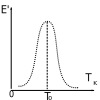
\includegraphics[scale=1]{fero1.svg}
$T_K$ - temperatūra kelvino skalėje
$T_0$ - temperatūra Kiuri
$\varepsilon'$ - dielektrinė skvarba
Jei fero elektrinėje fazėje fero elektrikas turėjo polinę simetriją,
tai paraelektrinėje fazėje medžiaga tampa nepolinė
(gardelė įgyja simetrijos centrą)

\textbf{2-tros rūšies fazinis virsmas}:
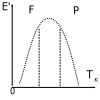
\includegraphics[scale=1]{fero2.svg}
Vyksta kitimas iš $F$ero elektrinės į $P$ara elektrinę fazę.

Visais atvejais fero-elektriką nusako Kiuri dėsnis
$\varepsilon = \varepsilon_{\infty} - \frac{C}{T - T_K}$
$\varepsilon_{\infty}$ - lūžio rodiklio kvadratas \textit{(?)},
dielektrinė skvarba, kuri yra elektroninės poliarizacijos matas \textit{(?)}.
$C$ - konstanta

Jei vyksta 1-mos rūšies faziniai virsmai,
tai C $\approx (10^3 - 10^4) deg$

Jei 2-tros rūšies ─ C $\approx (10^2 - 10^3) deg$

Jei atvaizduotume $\frac{1}{\varepsilon}$

...

\begin{remember}
	\item Kas yra feroelektrikai
	\item Kad fero elektrinėje fazėje reiškiasi domeninė struktūra
	\item Faziniai virsmai (1-mos, 2-tros rūšies)
	\item Koks dėsnis aprašo (Kiuri)
	\item Dielektrinė skvarba (1-mos, 2-tros rūšies) nuo temperatūros
	\item Faziniai virsmai (Landau) (1-mos, 2-tros rūšies)
	\item Kaip kinta spontaninė poliarizacija (1-mos, 2-tros rūšies)
	\item Dielektrinė skvarba priklauso nuo elektrinio stiprio (P ir F)
	\item Poliarizacija patalpinant į periodinį lauką (P ir F; Histerizė)
\end{remember}

\section{Diamagnetikai, paramegnetikai, feromagnetikai magnetiniame lauke.}
Feromagnetikų visi netiesiniai parametrų kitimai yra valdomi magnetiniais
laukais. Nagrinėsime, kaip kinta magnetinio lauko indukcija, nuo
lauko stiprio. Kaip valdoma magnetinė skvarba magnetiniais laukais.
Histerizės reiškinys. Kam tinka praktikoje feromagnetikai. Iš
feromagnetinės fazės į … Kuri, Lažavenas. Diamagnetikai – medžiagos, kurių
magnetinis momentas yra 0. (Pavyzdžiui, oras.)


\subsection{Feromagnetikai}

Feromagnetikų kilomodinis … yra didžiausias lyginant su
paramagnetikais ir diamagnetikais. Feromagnetikai tai yra medžiagos,
kurios priklausomai nuo temperatūros, gali būti vienoje iš dviejų
fazių: feromagnetinėje arba paramagnetinėje fazėje. Tai yra
feromagnetikuose, priklausomai nuo temperatūros, vyksta fazinis virsmas
iš feromagnetinės į paramagnetinę fazę. Feromagnetinėje fazėje
egzistuoja domeninė struktūra. Feromagnetikuose domenai, tai yra
sritys, turinčios tam tikros krypties, magnetinę indukciją.
Magnetinė indukcija yra žymima raide $B$. Sąryšis tarp magnetinės
indukcijos ir magnetinio lauko stiprio yra $B = \mu\mu_{0}H$.
$H$ yra matuojamas $\left[ \frac{A}{m} \right]$, $\mu$ – bedimensinis
dydis, o $\mu_{0} = 4 \pi \cdot 10 ^{-7}\frac{H}{m}$. Taigi
magnetinė indukcija yra matuojama teslomis $T$. Jeigu talpiname
feromagnetiką į magnetinį lauką ir didiname magnetinio lauko stipri,
tai esant tam tikram magnetinio lauko stipriui $H$ visi domenai išsidėstys
lauko kryptimi. Koercinis laukas (žymimas $H_{c}$) – lauko stipris,
kuriam esant orientuojasi visi domenai pagal išorinio lauko kryptį.
Gaunama monodomeninį (?) atvejį. Ši situacija yra įmanoma tik tada,
kai feromagnetikas yra feromagnetinėje fazėje.

% TODO: \mu priklausomybė nuo T (absoliučiosios temperatūros).
$T_{c}$ – temperatūra fazinio virsmo iš feromagnetinės į paramagnetinę
fazę.

% TODO: B priklausomybė nuo T.
Paramagnetinėje fazėje išnykstant domeninei struktūrai indukuotų
sričių magnetinė indukcija sumažėja iki 0.

% TODO: \mu priklausomybė nuo H.
Didėjant magnetinio lauko stipriui, magnetinė skvarba, iki tam tikros
magnetinio lauko stiprio reikšmės $H_{c}$ didėja, o vėliau didėjant
magnetinio lauko stipriui, feromagnetiko magnetinė skvarba mažėja.
(Ši priklausomybė yra galima tik tada, kai feromagnetikas yra 
feromagnetinėje fazėje.)
Priežastis: didėjant lauko stipriui vis daugiau ir daugiau domenų
orientuojasi magnetinio lauko kryptimi ir dėl šitos priežastis
magnetinė indukcija didėja ir savo ruožtu didėja magnetinė
skvarba.
\begin{align*}
  \mu &= \frac{B}{\mu_{0}H} & B = const\t{, kai} H \geq H_{c} \\
\end{align*}
Esant koerciniam laukui $H_{c}$ feromagnetikas tampa monodomeniniu ir
toliau didėjant magnetinio lauko stipriui, indukcija $B$ lieka konstanta.

%TODO: \mu priklausomybė nuo H, kai feromagnetikas yra paramagnetinėje
% fazėje (primena 1/x grafiką).

%TODO: B priklausomybė nuo H, kai talpiname į periodinį lauką.
% (Feromagnetinėje fazėje.)
Ši kreivė yra vadinama Histerezės kilpa.

%TODO: B priklausomybė nuo H, kai talpiname į periodinį lauką.
% (Paramagnetinėje fazėje.)
Paramagnetiko indukcija yra tiesinė jo magnetinio lauko stiprio
funkcija.

Svarbu:
\begin{itemize}
  \item kas yra būdinga feromagnetikams (kad jie priklausomai nuo
    temperatūros gali būti arba feromagnetinėje arba paramagnetinėje
    fazėje);
  \item vyksta fazinis virsmas iš feromagnetinės į paramagnetinę;
  \item domenai
  \item kaip kinta magnetinė skvarba priklausomai nuo T ir H;
  \item kaip kinta H nuo T;
  \item mokėti paaiškinti, kodėl yra tokia $\mu$ priklausomybė nuo H;
  \item kas darosi, jei feromagnetiką talpiname į periodinį magnetinį
    lauką.
\end{itemize}
Dažniausiai pasitaiko tik pirmos rūšies fazinis virsmas. (Bet pridėjus
priemaišų, galima gauti ir antros rūšies fazinė virsmą.)

\subsection{Paramagnetikai}

$C$ – Kiuri konstanta,
$T$ – temperatūra absoliučioje temperatūroje.

Įmagnetėjimas $\vec{I} = n_{0}\vec{p}_{m}L(a)$, čia
\begin{description}
  \item[$n_{0}$] – elektronų koncentracija;
  \item[$L(a)$] – klasikinė Lanžaveno funkcija,
    $L(a) = \coth a - \frac{1}{a}$.
\end{description}

Wėberis – magnetinio lauko linijų skaičius kertantis tam tikra ploto
vienetą.

Elektrono magnetinis momentas $p_{m} = \mu_{B}$.

Svarbu:
\begin{itemize}
  \item paramegnetikuose galime indukuoti magnetinį momentą esant
    tam tikriems lauko stipriams;
  \item kaip galima paskaičiuoti kilomolinį jautri remiantis Kuri
    formule;
  \item ką pasiūlė Lanžavenas;
  \item kaip galime surasti įmagnetėjimą, naudojantis dviem sąlygom
    kai magnetinio lauko energija yra žymiai mažesnė už šiluminę
    energiją, ir, kai magnetinio lauko energija yra žymiai didesnė
    už šiluminę energiją.
\end{itemize}

\subsection{Diamagnetikai}

Magnetikai, kuriuose negalima indukuoti magnetinio momento.

$\Xi_{kmol}$ – kilomagnetinis jautris?

Paprasčiausias iš diamagnetikų pavyzdys yra oras.

Kontroliniam darbe bus po 3 skirtingus klausimus. Bus 5 skirtingos
grupės. Atsinešti rašiklį ir savo smegenis.

\section{Superjonikai.}
Medžiagos, kuriose pagrindiniai krūvininkai yra katijonai ir medžiagos
anijonai. Masės ir elektrinio krūvio perneša. Elektroninis laidumas yra
žymiai mažesnis už joninį. Superjonikais tas medžiagas vadina fizikai,
o kietojo kūno specialistai juos vadina kietaisiais elektrolitais.
Neišeina aprašyti Faradėjaus dėsniais. Yra naudojamos … taškinio teorijos.
\section{Superlaidininkai.}
Skirstomi į dvi grupes:
\begin{itemize}
  \item žematemperatūriai – fazinis virsmas į superlaidžią būsena virsta
    4-6 K temperatūroje;
  \item aukštatemperatūriai – skysto azoto temperatūroje.
\end{itemize}
Meisnerio efektas – iš medžiagos yra išstumiamas magnetinis laukas.
(Jei patalpinsim medžiagą virš magneto ir sukelsim superlaidumą,
tai …)
